\subsection{Long-form Hallucination Detection}
\label{sec:longform}

\begin{table*}[t]
\centering
\caption{\textbf{Long-form hallucination detection --- token level.} We
report AUROC per (LLM, dataset) cell. Models: Mistral-7B-Instruct-v0.2
(Mis-7B-Inst), Llama-3.1-8B-Instruct (LlaMa-8B-Inst),
Llama-3.1-70B-Instruct (LlaMa-70B-Inst). Datasets: RAGTruth
\citep{niu2024ragtruth}, FactScore \citep{min2023}, LongFact
\citep{wei2024}. Per-token gold mask built from atom spans via
longer-span-wins on containment, earlier-span-wins on partial overlap;
uncovered tokens dropped. Best score per column in \textbf{bold},
second-best \underline{underlined}. $^\dagger$ marks cells whose data
comes from a closely related model version
(Mistral-7B-Instruct-v0.1 for RAGTruth, Llama-3-8B-Instruct for
LongFact). Cells with ``---'' indicate experiments not yet run.}
\label{tab:main}
\setlength{\tabcolsep}{2.5pt}
\renewcommand{\arraystretch}{1.05}
\scriptsize
\adjustbox{max width=\textwidth}{%
\begin{tabular}{l ccc ccc ccc}
\toprule
 & \multicolumn{3}{c}{Mis-7B-Inst} & \multicolumn{3}{c}{LlaMa-8B-Inst} & \multicolumn{3}{c}{LlaMa-70B-Inst} \\
\cmidrule(lr){2-4} \cmidrule(lr){5-7} \cmidrule(lr){8-10}
Method & RAGTruth & FactScore & LongFact & RAGTruth & FactScore & LongFact & RAGTruth & FactScore & LongFact \\
\midrule
SemanticEntropy           & --- & --- & --- & --- & --- & --- & --- & --- & --- \\
DegMat (NLI)              & --- & --- & --- & --- & --- & --- & --- & --- & --- \\
EigValLaplacian (NLI)     & --- & --- & --- & --- & --- & --- & --- & --- & --- \\
SAR                       & --- & --- & --- & --- & --- & --- & --- & --- & --- \\
LUQ                       & --- & --- & --- & --- & --- & --- & --- & --- & --- \\
KernelLanguageEntropy     & --- & --- & --- & --- & --- & --- & --- & --- & --- \\
\midrule
Perplexity                & --- & --- & --- & --- & --- & --- & --- & --- & --- \\
MeanTokenEntropy          & --- & --- & --- & --- & --- & --- & --- & --- & --- \\
MCNSE                     & --- & --- & --- & --- & --- & --- & --- & --- & --- \\
TokenSAR                  & --- & --- & --- & --- & --- & --- & --- & --- & --- \\
\midrule
CocoaMSP                  & --- & --- & --- & --- & --- & --- & --- & --- & --- \\
CocoaPPL                  & --- & --- & --- & --- & --- & --- & --- & --- & --- \\
CocoaMTE                  & --- & --- & --- & --- & --- & --- & --- & --- & --- \\
\midrule
Act-ViT (F-v2, N\textsubscript{eff}=6)
                          & \underline{0.570}$^{\dagger}$ & \underline{0.676} & \underline{0.638} & --- & \textbf{0.673} & \underline{0.578}$^{\dagger}$ & --- & --- & --- \\
Temp-ViT (Stage 3, ours)  & \textbf{0.865}$^{\dagger}$ & \textbf{0.696} & \textbf{0.692} & --- & \underline{0.653} & \textbf{0.601}$^{\dagger}$ & --- & --- & --- \\
\bottomrule
\end{tabular}%
}
\end{table*}


The long-form setting is reported at three granularities on RAGTruth
\citep{niu2024ragtruth}, FactScore \citep{min2023}, and LongFact
\citep{wei2024}. Table~\ref{tab:main} reports the headline
token-level numbers; Table~\ref{tab:sentence} reports
sentence-level verdicts under AND-on-supported aggregation
(any unsupported atom in a sentence flips the sentence to
hallucinated, score is the max per-token uncertainty in the span);
Table~\ref{tab:claim} reports claim-level verdicts (one row per
atomic fact). Temp-ViT denotes the full three-stage pipeline; at each
granularity the score is the per-token sigmoid of the Stage-3
detector aggregated over the relevant span. The patterns answer
(Q\textsubscript{1}): the gap to the Act-ViT pooled tensor baseline
widens as the granularity narrows (claims), where the head must rank
atoms against each other within the same passage.
Table~\ref{tab:long_form_stats} reports the passage- and atom-length
distributions that determine which granularity is feasible to
supervise; LongFact and FactScore atoms are typically much shorter
than RAGTruth's, which the per-token head benefits from.

\paragraph{Run-time and performance trade-offs.} Temp-ViT scores
every generated token in a single forward through the frozen encoder
and the Mamba-2 head, so the cost of obtaining sentence- or
claim-level scores is amortized across the passage rather than
scaling with the number of claims. Figure~\ref{fig:inference_time}
quantifies this on a $T = 384$ LongFact passage: roughly an order of
magnitude wall-clock advantage over sequence-level activation-tensor
baselines that must be re-invoked per claim. Training the
passage-level refinement stage takes under three hours on a single
H200 across all three LLMs. Aggressive pooling
($(L_p, N_p) = (4, 20)$) preserves most of the per-atom AUROC while
shrinking training to a few minutes.

\begin{figure}[t]
\centering
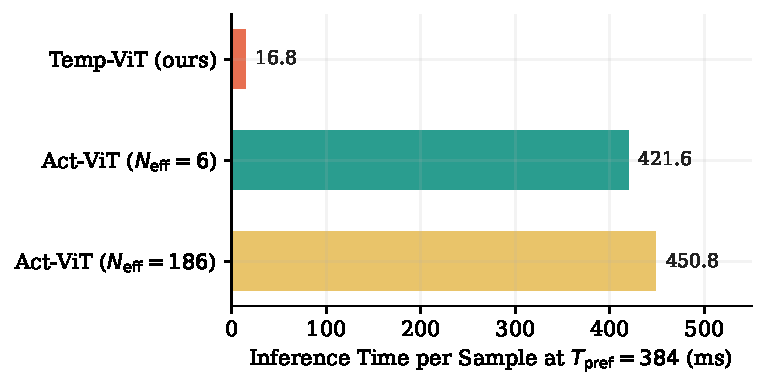
\includegraphics[width=0.95\linewidth]{figs/fig_inference_time.pdf}
\caption{Wall-clock time to score every token of one $T = 384$-token
LongFact passage on a single H200, batch~1, FP32. ACT-ViT emits one
scalar per call, so labelling every token requires $T$ sequential
forwards; per-call latency is small but the total scales linearly with
the response length, even when the post-pool ViT input is widened to
recover long-range accuracy (\emph{N\textsubscript{eff}=186}).
Temp-ViT produces the full per-token logit vector in a single forward
pass and is roughly $25\times$ faster on this passage, illustrating
the real-time-cost weakness of activation-tensor methods that need one
call per generated token.}
\label{fig:inference_time}
\end{figure}

